\documentclass{article}

% Language setting
% Replace `English' with e.g. `Spanish' to change the document language
\usepackage[english]{babel}

% Set page size and margins
% Replace `letter paper' with `a4paper' for UK/EU standard size
\usepackage[letterpaper,top=2cm,bottom=2cm,left=3cm,right=3cm,marginparwidth=1.75cm]{geometry}

% Useful packages
\usepackage{amsmath}
\usepackage{graphicx}
\usepackage{algorithm}
\usepackage{hyperref}
\usepackage{algpseudocode}
\usepackage[colorlinks=true, allcolors=blue]{hyperref}
\usepackage{graphicx}

\title{New regression model research}
\author{David Sasaki}

\begin{document}
\maketitle

\section{Introduction}

The purpose of this paper is to build the best-performing deep learning model to predict bond prices.\\
\\
We've already designed the ResidualNN model to predict bond prices. Residual neural networks are used to predict bond prices by using the historical trace data of bond prices to train the network. The network should be able to extract the underlying trends and patterns from the data, which can then be used to make more accurate predictions about future bond prices. In addition, residual networks can also be used to detect anomalies in the data, which can help identify potential risks associated with investing in bonds.\\
\\
We are going to improve the performance by adding a new dataset and changing the architecture of the existing ResidualNN.

\section{Related Work}

There are several common approaches for processing time series financial data.\\
\\
1. \href{https://www.atlantis-press.com/proceedings/kam-15/25464}{Kalman Filters}: Kalman filters are a type of mathematical algorithm that can be used to build a regression model. The Kalman filter works by taking a set of observations and predicting a future value based on the previous values. In a regression model, Kalman filters are used to predict the next value of a given data set by taking into account the current state of the data and any previous observations.\\
\\
Advantage: The filter can be used to model both linear and non-linear systems.\\
Disadvantage: The filter is sensitive to initial conditions and can be difficult to debug.\\
\\
2. \href{https://link.springer.com/article/10.1007/s11403-021-00342-5}{Autoregression}: Autoregression is a type of regression analysis that uses historical values of a single variable to predict future values of that same variable. It is a type of linear regression model used to predict future values from past values. Autoregression models assume that the future values of the variable are linearly dependent on its past values. Autoregression models are used to predict trends in time series data, such as sales, economic cycles, and stock prices. Autoregression models can also be used to identify and remove trends in data.\\
\\
Advantage: Autoregression models are relatively simple and easy to use.\\
Disadvantage: Autoregression models can be overly simplistic and fail to capture non-linear relationships between variables.\\
\\
3. \href{https://www.sciencedirect.com/science/article/pii/S2210832714000258}{ARIMA}: ARIMA stands for AutoRegressive Integrated Moving Average. It is a type of regression model used for time series forecasting. The model uses past data to make predictions about future data. It is a combination of two models: autoregression (AR) and moving average (MA). AR models the effects of past observations on the current value, while MA models the effects of current errors on future values. The “integrated” part in ARIMA stands for differencing, which is used to make the data stationary. Stationary data has a constant mean and variance over time, making it easier to model. The model also uses parameters to determine the order of the AR and MA components, as well as the strength of the seasonal component, if present. By using historical data, ARIMA provides an efficient way to forecast future values.\\
\\
Advantage: ARIMA models are flexible and can be adapted to different types of time series data.\\
Disadvantage: ARIMA models can be difficult to tune and optimize.\\
\\
4. \href{https://www.sciencedirect.com/science/article/pii/S1877050920304865}{Long Short-Term Memory (LSTM) Networks}: LSTMs are a type of recurrent neural network that are designed to better capture long-term dependencies in time series data, making them well-suited to processing financial data.\\
\\
Advantage: LSTMs are well-suited to processing long-term dependencies in time series data.\\
Disadvantage: Training LSTM models is difficult, as the gradient of the error surface can be difficult to calculate. Furthermore, the vanishing gradient problem can cause problems in training LSTMs, as the gradient can become too small to be useful.\\
\\
5. \href{https://ieeexplore.ieee.org/abstract/document/4059381}{WaveNet}: WaveNets are a type of deep neural network architecture that is specifically designed for processing time series data. They are capable of extracting patterns from long sequences of data, making them suitable for financial data processing.\\
\\
Advantage: WaveNets are capable of extracting patterns from long sequences of data.\\
Disadvantage: Wavenet regression models are not capable of handling large datasets, as the model needs to be retrained for each new dataset.\\
\\
6. \href{https://www.sciencedirect.com/science/article/abs/pii/S0957417419301915}{CNNs}: CNNs (Convolutional Neural Networks) regression models are a type of neural network that is used to predict a continuous output. Unlike classification problems, where the output is a discrete label, regression problems predict a continuous output. CNNs are used for regression problems as they are able to identify patterns in the data. CNNs use convolutional layers, which are a type of neural network layer that is used to detect patterns in the data. Convolutional layers can detect patterns in the data that are not easily detected by traditional regression models. CNNs are also able to capture spatial relationships in the data, which is important for regression problems. Finally, CNNs are able to learn from data that is structured in a way that is not easily understood by traditional regression models.\\
\\
Advantage: CNNs are able to capture spatial relationships in the data, which is important for regression problems.\\
Disadvantage: CNNs can be computationally expensive, as they require large amounts of data and computation power.\\
\\
\\
These approaches are widely used for processing time series financial data. But they have their own disadvantages. The perfect bond price prediction model should possess the following requirements:\\
\\
1. Accurate and reliable data: The model should be fed with accurate, comprehensive, and up-to-date data.\\
\\
2. Robustness: The model should be able to handle different market conditions and scenarios.\\
\\
3. Flexibility: The model should be able to adapt to changing market conditions and regulations.\\
\\
4. Transparency: The model should be transparent and explainable, so users can understand the underlying assumptions and logic.\\
\\
5. Scalability: The model should be able to scale up in terms of complexity and the amount of data it can process.\\
\\

\section{Method}

At the moment, the ResidualNN model is the best one for the prediction. We have two plans to improve the accuracy.\\
\\
First, we can use the BondCliQ features. We want to add the BondCliQ features because we believe they will help the model price the bonds more accurately. Because the quotes that dealers are publishing will be highly correlated to where trades print. So, we will test the benefit when using BondCliQ data in experiments.\\
\\
Second, we are planning to add convolutional layers to the existing ResidualNN. We've already had both ResidualNN and SimpleConvolutionalNN. The new model we are going to build can be a combination of these two models. It means that we extract features from sequential trade features and quote features using convolutional layers, and then use those extracted features and RFQ features to predict bond prices using residual layers. So, we can combine CNN's advantages and ResidualNN's advantages to get the best results.\\
\\
We are not sure that the new model is better than the ResidualNN, so we are going to take several experiments. Since we are using MSE to estimate the accuracy, we are expecting an improvement in MSE. Finally, the goal of these experiments is to prove the benefit when using the BondCliQ features and adding convolutional layers.

\section{Experiments}

Since we only have the last four months of BondCliQ data, we will have experiments using the last four months of finra and BondCliQ data.

\subsection{Control Experiment: The Existing ResidualNN}

To compare the performance, we will have an experiment with the existing ResidualNN. We don't use BondCliQ features and Convolutional layers at this moment.

\begin{figure}
    \centering
    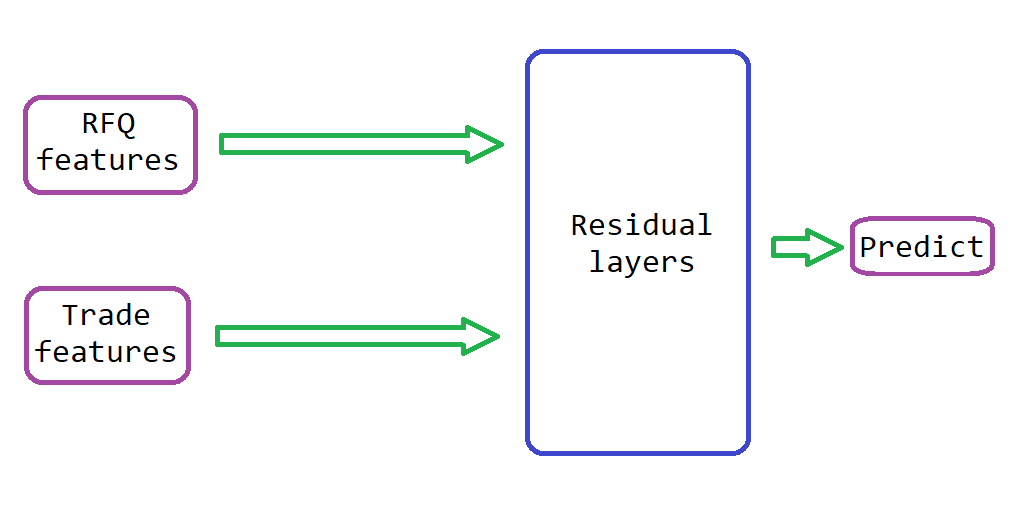
\includegraphics[scale=0.5]{NN-architecture-1.png}
    \caption{Control experiment network, the current Residual NN design}
    \label{fig:my_label}
\end{figure}

\subsection{Test the benefit when using BondCliQ data}

The second experiment is to test the benefit when using BondCliQ data. From BondCliQ data, we've already added quote features to batches.\\
\\
Adding more features can help a deep learning model to better capture the underlying patterns in the data, leading to increased accuracy. It can also help a deep learning model to better generalize to unseen data, leading to better performance on unseen data points. But sometimes, deep learning models are prone to overfitting when more features are added. Sometimes, as more features are added, it becomes harder to interpret the results of the model, and it may be difficult to understand the relationships between the features and the model’s output.\\
\\
Since the bond prices are relative to each other, we can normalize the batches using previous prices. We can subtract EMA (exponential moving average) or last prices from all of the trade prices. We also consider the relative time of the quote to the RFQ time.\\
\\
So, we are going to test the advantages when using BondCliQ data using the ResidualNN.\\
\\
In the existing ResidualNN, we only use RFQ and trade features. Because of this, we must modify the existing model for quote features. First, we get embedded features from quote features using ordinals. The input of the model is a combination of RFQ features, trade features, and quote features. Residual layers can predict bond prices by using historical features to extract the underlying trends and patterns from the data, which can then be used to make more accurate predictions about future bond prices.\\
\\
If there is an improvement in MSE after training the new model, we can realize the benefit when using the BondCliQ data.\\

\begin{figure}
    \centering
    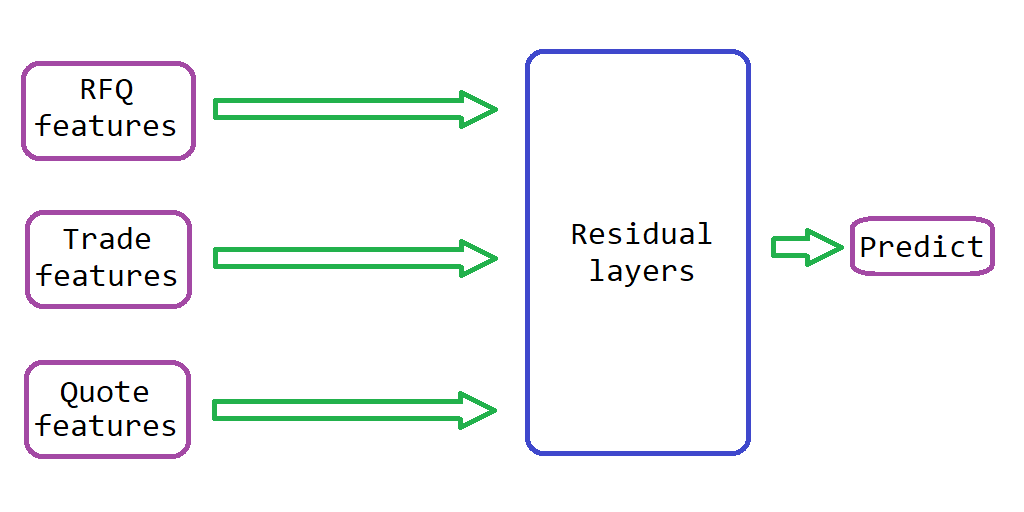
\includegraphics[scale=0.5]{NN-architecture-2.png}
    \caption{Using BondCliQ features, a new Residual NN design}
    \label{fig:my_label}
\end{figure}

\subsection{Test benefit when using both BondCliQ features and Convolutional layers}

We have three types of features - RFQ features, trade features, and quote features. The existing ResidualNN and SimpleConvolutionalNN only use RFQ features and trade features. We must modify the existing architecture.\\
\\
First, we get the embedded features from the original features using ordinals. There are categorical data types (figi, cusip, industry, and so on) in the features. We have ordinals to convert categorical values to numerical values. Ordinals are a kind of mapping from categorical values to identifier codes.\\
\\
Because we need to convert discrete values into continuous vector representation using the Embedding layer. This allows for features to be related to each other and for similar features to have similar numerical representations. This makes it easier for a neural network to learn the relationships between features, which can help improve the performance of the model. These embed features are the input of the model.\\
We are going to embed the identifier code for the dealer sending the quote.\\
\\
Then, we add convolutional layers to extract features from sequential trade features and quote features. We use 1D convolutional layers. Convolutional layers are a fundamental building block in deep learning models. They are used to detect patterns in sequential features and extract features from them. A convolutional layer consists of a set of filters, which are used to detect patterns in the input data. The filters are convolved with the input data to generate feature maps. These feature maps are then used as input for the next layer.\\
\\
The convolutional layer is usually the first layer in a deep learning model. It computes features from the input sequential features and extracts important features from them. For example, in an image recognition task, the convolutional layer will extract features such as edges, shapes, and textures from the input images. This layer is then followed by other layers such as pooling layers and fully-connected layers, which build upon the features extracted from the convolutional layer.\\
The convolutional layer has many advantages over traditional fully-connected layers. It reduces the number of parameters, which makes training faster and more efficient. It also allows for the extraction of spatial information, which is important in many tasks such as object detection. Additionally, the convolutional layer can capture spatial correlations, which are important in many tasks.\\
\\
The convolutional layers use a set of kernels (also known as filters) to scan the input data and extract features from it. The kernels are usually small, square matrices that are multiplied with the input data to produce a feature map. This feature map is then passed onto the next layer for further processing. Kernel convolution is not only used in CNNs but is also a key element of many other algorithms. It is a process where we take a small slice of numbers (called kernel or filter), pass it over our sequential features and transform it based on the values from the filter. Subsequent feature map values are calculated according to the following formula, where the input is denoted by f and our kernel by h. The indices of rows and columns of the result vector are marked with n.\\
\\
Convolution is a mathematical operation on two functions $f$ and $g$ expressing how the shape of one is modified by the other.\\
\\
$(f*g)(t)=\int_{0}^{t} f(x)g(t-x) \,dx$\\
\\
For complex-valued functions f, g defined on the set Z of integers, the discrete convolution of f and g is given by:\\
\\
$(f*g)(n)=\sum_{m=-M}^{M} f[n-m]g[m]$\\
\\
We can use different kernel and window sizes. We can set the kernel size from 1 to 3, and the window size from 128 to 1024.\\
\\
In terms of activation function, we're going to use ReLU. ReLU (Rectified Linear Unit) is a commonly used activation function in deep neural networks. It is used to introduce non-linearity into the network, allowing the model to learn more complex representations of the data. ReLU takes the form of a function, where any input value that is less than 0 is set to zero and any input value greater than 0 is passed through unchanged.\\
\\
The formula is like the following.\\
\\
$f(x) = max(0, x)$\\
\\
And, there are also max pooling layers. Max pooling layers are a type of layers used in convolutional neural networks (CNNs). They are used to reduce the spatial resolution of an input, while retaining the features that are important for the prediction task. Max pooling works by taking the maximum value from a set of input values and outputting it as a single output value. By doing this, it reduces the size of the input while still keeping the important features. Max pooling layers are typically used after a convolutional layer to reduce the number of parameters in the network, and to reduce overfitting.\\
\\
Next, we add residual layers. They can effectively capture non-linear relationships. They are able to learn complex interactions between different features and complex transforms of the input data. They are also capable of handling large datasets with high dimensionality. So, they are often used to create powerful regression models.\\
\\
Residual layers consist of two parts: a linear transformation and a shortcut connection. The linear transformation part is used to learn the features of the data, while the shortcut connection allows for the addition of information from the previous layers. This helps reduce the difficulty of training deep networks by allowing for easier optimization of the parameters.\\
\\
We are expecting that this model performs better than the previous one. We're going to train this model, and calculate the MSE. If there is no benefit, we shouldn't use convolutional layers.\\
\\

\begin{figure}
    \centering
    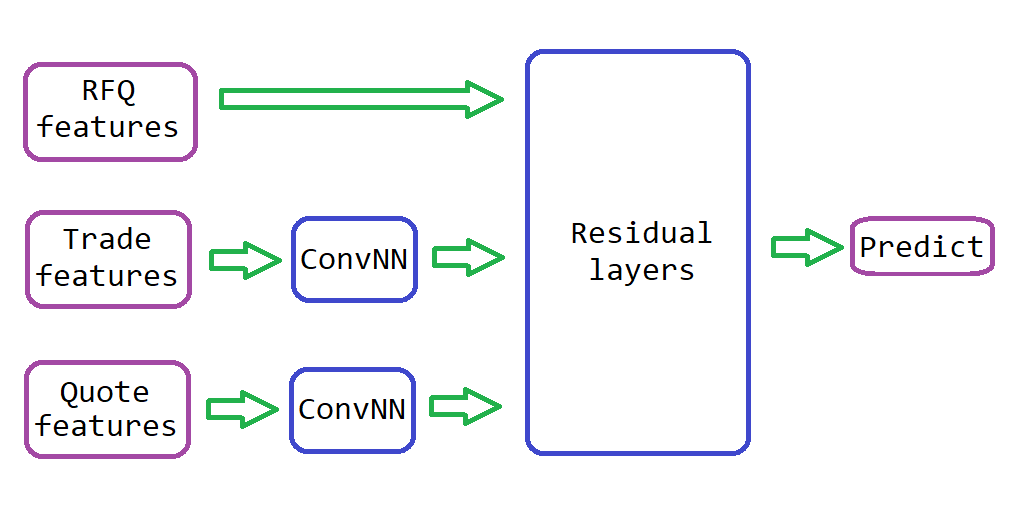
\includegraphics[scale=0.5]{NN-architecture-3.png}
    \caption{Using BondCliQ and Convolutional layers, final Residual NN design}
    \label{fig:my_label}
\end{figure}

\subsection{Summary}

Here is the summary of the experiments.\\

\begin{tabular}{ |p{2.5cm}|p{5cm}|p{5cm}|  }
\hline
\multicolumn{3}{|c|}{Experiments} \\
\hline
ResidualNN & ResidualNN with BondCliQ & ResidualNN with BondCliQ and Convolutional layers \\
\hline
Test Loss: & Test Loss: & Test Loss: \\
Memory: & Memory: & Memory: \\
Time: & Time: & Time: \\
\hline
\end{tabular}

\section{Conclusion}

If there is an improvement in terms of the new models, we can decide to use the BondCliQ data and change the model's architecture.\\

\\
\begin{thebibliography}{9}

\bibitem{reference1}
Xu Yan, Zhang Guosheng (2015), Application of Kalman Filter in the Prediction of Stock Price

\bibitem{reference2}
Xin-Zhou Qi, Zhong Ning, Meng Qin  (2021), Economic policy uncertainty, investor sentiment and financial stability—an empirical study based on the time varying parameter-vector autoregression model

\bibitem{reference3}
C. Narendra Babu, B. Eswara Reddy  (2014), Prediction of selected Indian stock using a partitioning–interpolation based ARIMA–GARCH model

\bibitem{reference4}
Adil Moghar, Mhamed Hamiche  (2020), Stock Market Prediction Using LSTM Recurrent Neural Network

\bibitem{reference5}
M. Rashidi-Nejad, A. Gharaveisi, M. R. Salehizadeh  (2006), Eelctricity Price Forecasting Using WaveNet

\bibitem{reference6}
Ehsan Hoseinzade, Saman Haratizadeh  (2019), CNN-based stock market prediction using a diverse set of variables

\end{thebibliography}

\end{document}